\begin{seanceprof}[Étude qualitative de fonctions]

\Titre{Description d'un comportement}{1}
\end{seanceprof}

\begin{CpsCol}
\textbf{Variations de fonctions}
\begin{description}
\item[$\square$] Décrire avec un vocabulaire adapté ou un tableau de variation le comportement d'une fonction définie par une courbe
%\item[$\square$] Dessiner une représentation graphique compatible avec un tableau de variation
\item[$\square$] Dessiner le tableau de variations d'une fonction dont on connait la courbe
\end{description}
\end{CpsCol}


\begin{tabular}{|c|c|c|}
\hline 
Modalité spatiale & Modalité temporelle & Modalité collaborative \\ 
\hline 
Présentiel & Synchrone & Binôme \\ 
\hline 
\end{tabular} 
% Modalité spatiale : Présentiel - Distanciel
% Modalité temporelle :  Synchrone ou Asynchrone
% Modalité collaborative : Individuelle - Binome - groupe - classe


\subsubsection{Activité apprenant}

\begin{description}
\item[Consigne(s)]  Faire l'activité 

\item[Matériel pédagogique] Fiche élève 

\item[Complément] 

\end{description}


\subsubsection{L'activité décryptée - Compétences visées}

\begin{description}
\item[1. Représenter - Communiquer.] 
Rappel du vocabulaire : Image, antécédent, fonction. Introduction de minimum, maximum.
Pour la justification, les valeurs de AG pour $x=0$, $x=3$ ou $x=5$ sont satisfaisantes.
\item[2. Représenter - Communiquer.] 
Amener l'élève à formaliser la difficulté d'écrire par des phrases le comportement de la fonction. L'utilisation d'un tableau de variations est une bonne alternative pour décrire le comportement.
%\item[3. Calculer.] 
%Formaliser une fonction par son expression et montrer que la courbe est la représentation de la fonction. L'utilisation de GGB pour tracer la fonction est privilégiée. 
%
%\textbf{Coup de pouce :}  Indiquer si besoin qu'il est toujours intéressant d'utiliser un point "annexe", ici le point H tel que GOH soit un triangle rectangle en H.
%\item[4. Représenter : Changer de registre.] 
%Lorsque $G$ appartient à $[AB]$, tous les points du segment sont inclus dans le disque de rayon 3. L'élève fait la correspondance entre les points à l'intérieur du cercle et les points de la courbe dont l'ordonnée est inférieure à 3. Cette question valide aussi la question 1.
%\item[5. Calculer.] Cette question est traitée par les plus avancés.
\item[3. Représenter - Raisonner.]
Cette question met en lumière la notion de courbe point par point. Le raisonnement sur le segment [Ab] est poursuivi sur la suite du trajet du gardien. Cette question permet de valider la compréhension des élèves sur la question 1.

\end{description}

\subsubsection{Activité Enseignant}

\begin{enumerate}
\item 
\begin{enumerate}
\item Après avoir établi l'appel, faire inscrire sur le cahier le thème d'étude : "\textbf{Étude quantitative de fonctions}"
\item Expliciter les grandes lignes du thème. Connaissances ci-dessus.
\item Distribuer l'activité. \textit{Pour la distribution, il est possible de donner la l'ensemble des feuilles à un premier élève qui transmet le paquet au voisin et de proche en proche, la distribution s'opère.}
\item Vidéo-projeter et présenter \textbf{brièvement} l'activité.
\item Passer dans les rangs pour jauger le travail des binômes.
\item Faire une synthèse générale au tableau, au besoin envoyer un élève.
\end{enumerate}
\item Faire émerger l'utilisation du tableau de variation. Cette question dure 10 minutes. Les élèves doivent être confrontés à des difficultés et/ou des imprécisions en utilisant des phrases. Amener le tableau de variations.
\item S'assurer que les élèves ont compris que sur l'intervalle [0;5], la courbe est la copie de la courbe de la question 1. Faire une synthèse avec un élève au tableau.\\
On appuiera l'idée que la courbe de la fonction est un ensemble de points. Lorsque l'élève complète le tracé, l'enseignant fait remarqué que l'élève place des points et que la juxtaposition de ces points construit la courbe.

\textbf{Avec la nouvelle forme du cycle 5 et l'évaluation au Baccalauréat des candidats par un grand oral, il est impératif que les élèves soient rompus aux oraux. Il faut veiller à pratiquer les restitutions orales devant public autant que possible, mais avec discernement.}


%\item \textbf{Coup de pouce :}  Indiquer si besoin qu'il est toujours intéressant d'utiliser un point "annexe", ici le point H tel que GOH soit un triangle rectangle en H. 
%
%\textbf{Coup de pouce :} Décomposer $[AB]$ en deux segments $[AH]$ et $[HB]$.
%
%La décomposition sur 2 intervalles peut être un frein à plusieurs élèves. Il ne faut pas hésiter à donner le coup de pouce.
%\item \textbf{Cette partie est réservée aux plus avancés}. Travail en autonomie.
%\item Conserver les 15 dernières minutes de la séance pour écrire une trace écrite. Les élèves créent leur trace écrite. S'assurer que les définitions ci-dessous apparaissent.
\end{enumerate}

\subsubsection{Trace écrite}

\begin{DefT}{Courbe}
Soit $f$ une fonction définie sur un intervalle I. \\
On appelle courbe de la fonction $f$, aussi appelée représentation graphique de $f$, l'ensemble des points $M$ du plan dont les coordonnées sont $(x,f(x))$, où $x$ parcourt le domaine de définition de $f$.
\end{DefT}

\begin{DefT}{Tableau de variations}\index{Tableau de variations}
Un tableau de variations d'une fonction $f$ est un tableau dans lequel l'étude synthétise
\begin{description}
\item[•] le domaine de définition de $f$ explicitement,
\item[•] les variations de $f$ à l'aide de flèches,
\item[•] les maximum et minimum.
\end{description} 

\begin{tikzpicture}
\tkzTabInit[lgt=2,espcl=3]{ $x$ / 1,$f$  / 2}
{ $0$ ,$3$,$5$}
\tkzTabVar{+/$3$,-/$1$,+/$2$ }
\end{tikzpicture}
\end{DefT}


\begin{Rq}
La courbe représentative d'une fonction $f$ et le tableau de variations de $f$ correspondent.
\end{Rq}


\begin{DefT}{Variations - Approche visuelle}
Dans un tableau de variations,
\begin{description}
\item[•] Une fonction croissante sur un intervalle est représentée par une flèche qui monte sur cet intervalle.
\item[•] Une fonction décroissante sur un intervalle est représentée par une flèche qui descend sur cet intervalle.
\end{description}
\end{DefT}

%%%%%%%%%%%%%%%%%%%%%%%%% Séance 2

\begin{seanceprof}[Étude qualitative de fonctions]

\Titre{Applications}{1}
\end{seanceprof}

\begin{tabular}{|c|c|c|}
\hline 
Modalité spatiale & Modalité temporelle & Modalité collaborative \\ 
\hline 
Présentiel & Synchrone & Individuelle + Binôme \\ 
\hline 
\end{tabular} 
% Modalité spatiale : Présentiel - Distanciel
% Modalité temporelle :  Synchrone ou Asynchrone
% Modalité collaborative : Individuelle - Binome - groupe - classe


L'objectif de cette séance est de permettre à l'élève de fixer la notion de tableau de variation d'une fonction. L'enseignant restera attentif au fait qu'une fonction admet un unique tableau de variation mais à un tableau de variation donné, il existe une infinité de fonctions possibles.

Ces exercices sont une occasion de fixer le vocabulaire d'\texttt{image}, \texttt{antécédent}, \texttt{domaine de définition}, de revoir la notion de \texttt{fonction}.

La maitrise du vocabulaire, et \textit{a fortiori}, de l'utilisation des définitions formelles de \texttt{croissance} et \texttt{décroissance} est un attendu de fin d'année.


\begin{MEO}
Pour toute la séance, video-projeter la grille Geogebra avec le repère.
\end{MEO}


\subsection{Exercice par exercice}

\ExeComp{Représenter. Durée : 20 minutes}

Cet exercice d'application est l'occasion de rappeler le vocabulaire. On veillera à la construction de tableau de variation complet.

\subsection{Mise en oeuvre}

\begin{enumerate}
\item Faire travailler les élèves individuellement pendant 5-10 minutes sur les 2 premières courbes.
\item Au bout de ce temps, mettre les élèves par binôme pour une validation par pair\footnote{Le travail par les pairs est un travail entre personne de même rang ! Les élèves critiquent, évaluent, trouvent des solutions entre eux. Ce travail est réflexif.}. Cette phase permet l'autoévaluation et la prise de décision.
\item Envoyer au tableau un groupe qui pense être sûr des réponses pour chaque courbe. 
\item La courbe 3 doit permettre un tableau sans trop de difficulté. Le changement de variation sur 3 intervalles doit faire écho à la question 3 de l'activité 1.
\item La courbe 4 est la représentation d'une fonction définie sur $\R^*$. Il convient de faire attention et d'inscrire la double barre dans le tableau de variations. Il n'est pas nécessaire de s'étendre sur cette notion qui sera revue par la suite dans l'étude de domaine de définition.
\begin{Att}
\textbf{Note pour la formation des enseignants.}\\
Lorsque la courbe se dessine en levant le crayon ne signifie pas que la fonction n'est pas définie. La locution \textit{lever le stylo} est relié à la notion de continuité (en Terminale) et non au domaine de définition. Attention au terme employé.

On pourra faire écrire \textit{lorsqu'une valeur est \textit{interdite} sur un intervalle, le tableau de variations doit comporter une double barre pour signifier que cette valeur n'a pas d'image par la fonction étudiée.} 
\end{Att}
\end{enumerate}

Passer dans les rangs pour vérifier les tableaux.

\subsection{Trace écrite}

\begin{DefT}{Visualisation d'une fonction croissante ou décroissante}\index{Représentation graphique!Fonction croissante, décroissante}
\begin{description}[leftmargin=*]
\item[•] Lorsque, sur un intervalle $I$, la courbe représentative d'une fonction monte sans portion horizontale, on dit que la fonction est \textbf{strictement croissante sur $I$}. Si la courbe représentative possède une portion horizontale, on dit que la fonction est \textbf{croissante sur $I$}.
\item[•] Lorsque, sur un intervalle $I$, la courbe représentative d'une fonction descend sans portion horizontale, on dit que la fonction est \textbf{strictement décroissante sur $I$}. Si la courbe représentative possède une portion horizontale, on dit que la fonction est \textbf{décroissante sur $I$}.
\end{description}
\end{DefT}

%%%%%%%%%%%%%%%% Exercice 2 

\ExeComp{Représenter. Raisonner. Durée : 15 minutes}

Cet exercice d'application est l'occasion de fixer les notions écrites dans le cahier sur le lien entre variations et courbe.


\subsection{Mise en oeuvre}

\begin{enumerate}
\item Faire travailler les élèves par binôme 5-10 minutes.
\item L'enseignant trace une courbe au tableau qui répond à la consigne. Il y a fort à parier qu'aucun élève n'aura la même courbe que l'enseignant ! Envoyer un élève au tableau pour présenter et valider son tracé. Engager la discussion sur les courbes convenables.
\begin{Rq}
Il ne faut pas se laisser déborder par le temps !
\end{Rq}
\end{enumerate}

%%%%%%%%%%%%%%%% Exercice 3 

\ExeComp{Représenter.}

Il faut que les élèves produisent au moins les 2 premières courbes en regard des deux premiers tableaux. Il n'est pas nécessaire que l'ensemble de la classe finissent l'exercice.

Les fonction $u$ et $h$ peuvent être proposées en devoir à la maison pour les élèves les plus lents.

\begin{Ast}
Pour gagner en temps, il est possible faire une atelier à 4 élèves. Chaque élève trace une seule courbe et la commente à ses 3 autre camarades pour validation.
\end{Ast}


\begin{seanceprof}[Étude qualitative de fonctions]

\Titre{Comparaison d'images}{1}
\end{seanceprof}

\begin{tabular}{|c|c|c|}
\hline 
Modalité spatiale & Modalité temporelle & Modalité collaborative \\ 
\hline 
Présentiel & Synchrone & Individuelle \\ 
\hline 
\end{tabular} 
% Modalité spatiale : Présentiel - Distanciel
% Modalité temporelle :  Synchrone ou Asynchrone
% Modalité collaborative : Individuelle - Binome - groupe - classe



\ExeComp{Communiquer. Raisonner.}

L'exercice est un contextualisation de l'utilité des fonctions. La durée de cet exercice qui peut être fait individuellement ne doit pas excéder 15 minutes.

\begin{Rq}
Rappeler au besoin que perdre 10\% revient à multiplier par 0,9. Il n'est pas utile de passer plus de temps dessus mais une trace écrite peut faire l'objet de ce rappel. C'est une notion importante pour l'ensemble des élèves sur la proportionnalité qui est utile dans toutes les séries du cycle terminal.
\end{Rq}

\ExeComp{Représenter. Communiquer.}

\textbf{Coup de pouce} : Tracer \textbf{une} figure qui correspond à ce tableau de variation.

\begin{Att}
On insiste bien sur le déterminant indéfini \textbf{une} et non pas \textbf{la}. Il faut que l'élève commence à percevoir la puissance du vocabulaire et sa rigueur dans l'apprentissage des mathématiques. 
\end{Att}

\begin{Att}
On insiste sur le fait qu'un minimum est unique. On dit alors le minimum. Attention dans la question , "un" a valeur de déterminant cardinal. 
\end{Att}

\subsubsection{Trace écrite}

\begin{DefT}{Maximum, minimum}
On dit que
\begin{description}[leftmargin=*]
\item[•] $M$ est le maximum de $f$ sur son domaine de définition si pour tout réel $x$ de $I$, $f(x) \leq M$. 
\item[•] $m$ est le minimum de $f$ sur son domaine de définition si pour tout réel $x$ de $I$, $f(x) \geq m$. 
\end{description} 
On dit que $f$ est bornée  sur $I$ lorsque $f$ accepte un maximum \textbf{et} un minimum sur $I$.
\end{DefT}



\ExeComp{Représenter. Communiquer.}


L'intérêt de cet exercice réside dans la formalisation des définitions de fonction croissante sur I et fonction décroissante sur I.


\subsubsection{Trace écrite}

Une première définition est 

\begin{DefT}{Fonction croissante, décroissante sur $I$}
On dit que
\begin{description}[leftmargin=*]
\item[•] une fonction $f$ est \textbf{croissante sur $I$}, lorsque les images de $a$ et de $b$ sont rangées dans le même ordre que $a$ et $b$.
\item[•] une fonction $f$ est \textbf{décroissante sur $I$}, lorsque les images de $a$ et de $b$ sont rangées dans l'ordre inverse de $a$ et $b$.
\end{description} 
\end{DefT}

qui peut amener la définition formelle. 

\begin{DefT}{Fonction croissante, décroissante sur $I$}
\begin{description}[leftmargin=*]
\item[•] une fonction $f$ est \textbf{croissante sur $I$}, lorsque pour tout nombre $a$ et $b$ de $I$ tels que $a \leq b$, $f(a) \leq f(b)$.
\item[•] une fonction $f$ est \textbf{strictement croissante sur $I$}, lorsque pour tout nombre $a$ et $b$ de $I$ tels que $a \leq b$, $f(a) < f(b)$.
\item[•] une fonction $f$ est décroissante sur $I$, lorsque pour tout nombre $a$ et $b$ de $I$ tels que $a \leq b$, $f(a) \geq f(b)$.
\item[•] une fonction $f$ est décroissante sur $I$, lorsque pour tout nombre $a$ et $b$ de $I$ tels que $a \leq b$, $f(a) > f(b)$.
\end{description} 
\end{DefT}


\begin{Att}
Selon le niveau de la classe, la définition formelle peut être vu bien plus tard. La formalisation est un attendu de fin de Seconde.
\end{Att}


\begin{seanceprof}[Étude qualitative de fonctions]

\Titre{Applications}{1}
\end{seanceprof}

\begin{tabular}{|c|c|c|}
\hline 
Modalité spatiale & Modalité temporelle & Modalité collaborative \\ 
\hline 
Présentiel & Synchrone & Multiformat \\ 
\hline 
\end{tabular} 
% Modalité spatiale : Présentiel - Distanciel
% Modalité temporelle :  Synchrone ou Asynchrone
% Modalité collaborative : Individuelle - Binome - groupe - classe


L'objectif de cette séance est de permettre à l'élève de fixer les notions. 

Ces exercices sont une occasion de fixer le vocabulaire d'\texttt{image}, \texttt{antécédent}, \texttt{domaine de définition}, de revoir la notion de \texttt{fonction}, de \texttt{maximum}, \texttt{minimum}.



\subsection{Exercice par exercice}

\ExeComp{Représenter. Durée : 10 minutes}

Individuelle

La valeur de 3 n'est pas possible car la fonction $f$ est décroissante sur $[-2;-1]$ et croissante sur $[-1;1]$ donc elle admet un minimum local égal à $f(-1)$ donc $f(-1) \leq 2$.

Toute justification  \textbf{rigoureuse} donnée par un élève est préférable.

Au bout de 5 minutes, .

\ExeComp{Représenter. Durée : 10 minutes}


\begin{seanceprof}[Étude qualitative de fonctions]

\Titre{S'auto évaluer}{1}
\end{seanceprof}

\begin{tabular}{|c|c|c|}
\hline 
Modalité spatiale & Modalité temporelle & Modalité collaborative \\ 
\hline 
Présentiel & Asynchrone & Individuel \\ 
\hline 
\end{tabular} 
% Modalité spatiale : Présentiel - Distanciel
% Modalité temporelle :  Synchrone ou Asynchrone
% Modalité collaborative : Individuelle - Binome - groupe - classe



\begin{seanceprof}[Étude qualitative de fonctions]

\Titre{Applications}{1}
\end{seanceprof}

\begin{tabular}{|c|c|c|}
\hline 
Modalité spatiale & Modalité temporelle & Modalité collaborative \\ 
\hline 
Présentiel & Asynchrone & Binôme \\ 
\hline 
\end{tabular} 
% Modalité spatiale : Présentiel - Distanciel
% Modalité temporelle :  Synchrone ou Asynchrone
% Modalité collaborative : Individuelle - Binome - groupe - classe
